% IEEEtran submission draft for Paper I (ODD Core)
% Source (content): Paper_01_ODD_Core_English_Submission.md
% Bibliography: odd_references.bib (IEEEtran.bst)

\documentclass[conference]{IEEEtran}

\usepackage{cite}
\usepackage{amsmath,amssymb}
\usepackage{amsthm}
\usepackage{graphicx}
\usepackage{xcolor}
\usepackage{listings}
\usepackage{url}
\usepackage{xurl}
\usepackage[hidelinks]{hyperref}

\lstset{
  basicstyle=\ttfamily\footnotesize,
  breaklines=true,
  columns=fullflexible,
  frame=single
}

% Fig. caption label style (requested: "Figure 1." instead of "Fig. 1.")
\renewcommand{\figurename}{Figure}

% Theorem-like environments
\newtheorem{definition}{Definition}

% TikZ for vector figure
\usepackage{tikz}
\usetikzlibrary{positioning}

\begin{document}

\title{Output-Driven Development (ODD): Foundations of Artifact Legitimacy in AI-Native Software Engineering}

\author{\IEEEauthorblockN{Yi Fu}
\IEEEauthorblockA{ODDFounder\\
Email: \href{mailto:fuyi.it@live.cn}{fuyi.it@live.cn}}}

\maketitle

\begin{abstract}
Large Language Models (LLMs) make code generation abundant, but they also collapse the traditional control surface of software engineering: changes can be produced faster than humans can review, and responsibility no longer maps cleanly to authorship. We present Output-Driven Development (ODD), an artifact-centric governance workflow for AI-assisted development. ODD shifts approval from diffs to accepted outputs by binding each release artifact to (1) an acceptance contract, (2) an evidence bundle produced by layered checks (tests, adversarial probes, and mutation testing), and (3) a signed seal that records who accepted what and when. This turns acceptance into an auditable operation and focuses human attention on explicit decision points and exceptions. We provide a minimal vignette and an adoption checklist for practitioners.
\end{abstract}

\textbf{Practitioner Insights:}
\begin{itemize}
\item Shift control from code review to artifact acceptance: approve contracts, not diffs.
\item Make acceptance auditable: seal each artifact with contract + evidence hashes and a human sign-off.
\item Scale verification with layered checks and treat exceptions as first-class events.
\end{itemize}

\begin{IEEEkeywords}
Output-Driven Development, AI-Native Software Engineering, Software Governance, Artifact Legitimacy, Acceptance Contracts, Mutation Testing, Provenance, Accountability
\end{IEEEkeywords}

\section{Introduction}
\subsection{Background: the broken control surface}
Recent advances in large language models (LLMs) have fundamentally altered how software is produced \cite{bubeck2023sparks, chen2021codex}. Code generation systems such as Copilot and ChatGPT are no longer auxiliary tools; they increasingly act as \emph{primary producers} of executable artifacts.

However, while generation capability has advanced rapidly, the control structures of software engineering have not evolved accordingly. Traditional methodologies---including Agile, DevOps, Test-Driven Development (TDD), and Model-Driven Engineering (MDE)---implicitly assume that:
\begin{itemize}
\item source code is authored by humans,
\item reasoning about behavior is mediated through code inspection,
\item responsibility can be traced through authorship and commit history.
\end{itemize}

These assumptions no longer reliably hold in AI-assisted production.

As a result, modern software systems increasingly exhibit a paradoxical condition:
\begin{quote}
\textbf{Code is abundant, yet responsibility is diffuse.\\
Automation is powerful, yet control is fragile.}
\end{quote}

Recent developer surveys suggest that AI-assisted coding has reached critical mass, but verification and accountable acceptance have not kept up. For example, Stack Overflow's 2024 Developer Survey reports broad use (or planned use) of AI tools alongside a persistent trust gap in AI output \cite{stackoverflow2024survey}. Sonar's 2026 developer survey highlights what it calls a ``verification gap'' between low trust and inconsistent verification practices \cite{sonar2026verificationgap}. These signals suggest that the limiting factor is shifting from generation speed to verification and responsible acceptance.

\subsection{The core problem: loss of responsibility anchors}
The central challenge introduced by AI-assisted software generation is not correctness alone, but the erosion of \emph{responsibility anchors}.

In conventional workflows, responsibility is implicitly attached to the human author, the review process, or module ownership. In AI-assisted workflows, however:
\begin{itemize}
\item code may be generated, revised, and regenerated multiple times,
\item generation paths are opaque and non-deterministic,
\item multiple agents (human and AI) may contribute asynchronously.
\end{itemize}

Under such conditions, the question ``Who is responsible?'' becomes structurally ill-defined.

Existing responses largely attempt to restore control by:
\begin{itemize}
\item improving prompt engineering and synthesis-oriented practices \cite{austin2021programsynthesis},
\item adding more tests,
\item constraining models or sandboxing execution.
\end{itemize}

While useful, these approaches operate within the code-centric paradigm and therefore fail to address the deeper structural shift.

ODD is not a new prompt recipe, a new testing technique, or a repackaging of Design by Contract (DbC) \cite{meyer1992dbc}, TDD \cite{beck2002tdd}, CI quality gates, or software supply-chain signing \cite{torresarias2019intoto, openssf2023slsa, newman2022sigstore}. It is a change in the \emph{control surface}: the primary object of governance becomes the artifact and its acceptance boundary, and responsibility is anchored in explicit arbitration decisions rather than continuous code review \cite{bacchelli2013codereview}.



\subsection{Output-Driven Development (ODD): a paradigm shift}
To address the above challenges, we introduce Output-Driven Development (ODD), an artifact-centric methodology for AI-assisted software engineering.

ODD is founded on three core principles:
\begin{enumerate}
\item \textbf{Outputs as first-class entities.} Artifacts are explicitly specified, validated, and audited.
\item \textbf{Contracts before generation.} Acceptable output spaces are defined prior to any AI execution.
\item \textbf{Responsibility through arbitration.} Humans are positioned as contract reviewers and final arbiters, not routine implementers.
\end{enumerate}

Rather than attempting to eliminate human involvement, ODD concentrates human attention on irreducible decision points, while delegating routine generation and validation to AI systems.


\subsection{Output-Driven Development (ODD) in one figure}
\begin{figure}[t]
\centering
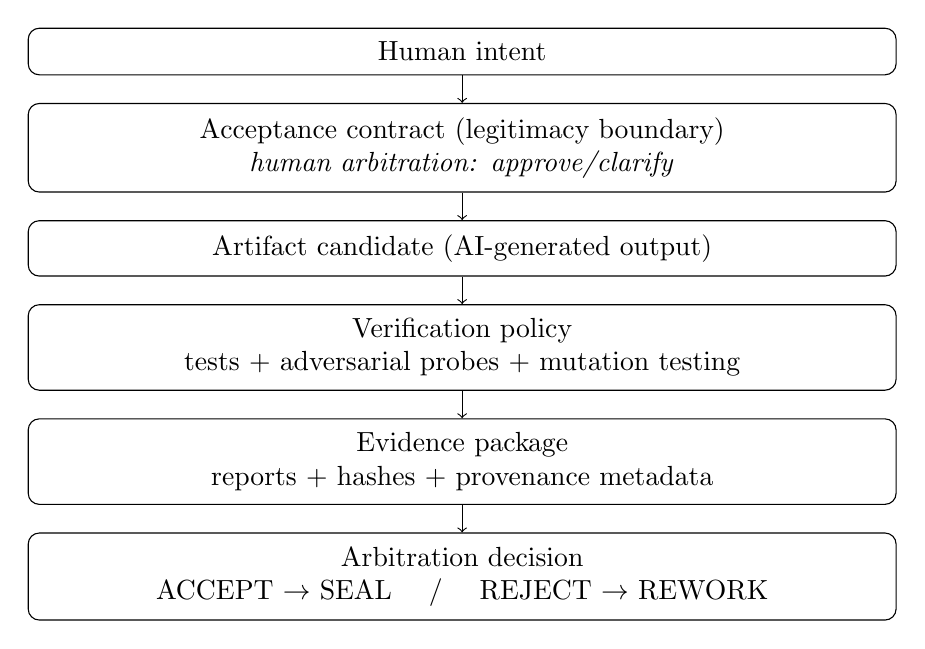
\begin{tikzpicture}[
  node distance=0.35cm,
  box/.style={draw, rounded corners, align=center, text width=0.88\columnwidth, inner sep=5pt}
]
\node[box] (intent) {Human intent};
\node[box, below=of intent] (contract) {Acceptance contract (legitimacy boundary)\\\emph{human arbitration: approve/clarify}};
\node[box, below=of contract] (artifact) {Artifact candidate (AI-generated output)};
\node[box, below=of artifact] (verify) {Verification policy\\tests + adversarial probes + mutation testing};
\node[box, below=of verify] (evidence) {Evidence package\\reports + hashes + provenance metadata};
\node[box, below=of evidence] (decision) {Arbitration decision\\ACCEPT $\rightarrow$ SEAL \quad / \quad REJECT $\rightarrow$ REWORK};

\draw[->] (intent) -- (contract);
\draw[->] (contract) -- (artifact);
\draw[->] (artifact) -- (verify);
\draw[->] (verify) -- (evidence);
\draw[->] (evidence) -- (decision);
\end{tikzpicture}
\caption{ODD control surface as artifact legitimacy.}
\label{fig:odd-control-surface}
\end{figure}

\subsection{Contributions}
This paper makes the following contributions:
\begin{enumerate}
\item \textbf{Control-surface reframing.} We define ODD as a shift in software governance: from code/process as the primary control unit to artifact legitimacy as the unit of acceptance.
\item \textbf{Responsibility anchoring via arbitration.} We make explicit the responsibility shift from authorship and routine code review to contract approval and artifact acceptance at well-defined decision points \cite{bacchelli2013codereview}.
\item \textbf{Operational and formal definitions.} We provide testable definitions of artifact, legitimacy, evidence package, and sealing, relating sealing to provenance/attestation concepts in software supply chain security \cite{torresarias2019intoto, openssf2023slsa, newman2022sigstore}.
\item \textbf{A minimal workflow + vignette.} We outline a lightweight workflow and a concrete vignette showing how ODD can ship a high-risk change without line-by-line code review.
\item \textbf{Implications and research agenda.} We summarize implications for practitioners and open research directions for contracts, verification economics, and governance under AI-assisted production.
\end{enumerate}

\subsection{Scope}
This article focuses on a practical control-surface shift and a pilotable workflow. Empirical validation with production data is left for future work.

\section{Core concepts}\label{sec:core-concepts}
\subsection{Artifact legitimacy as the unit of control}
In ODD, the unit of engineering control is not source code or development process steps, but the produced artifact---a verifiable output that satisfies a human need and has direct use-value.

An artifact is \emph{legitimate} when it is accepted under an explicit contract and backed by verifiable evidence (e.g., tests, mutation analysis, and auditable acceptance records). In other words: ODD optimizes for defensibility of outcomes, not readability of implementations.

\textbf{Key properties:}
\begin{itemize}
\item \textbf{Verifiable}: correctness can be checked against explicit criteria.
\item \textbf{Need-fulfilling}: it corresponds to an explicit human need (not an internal engineering activity).
\item \textbf{Use-value}: it can be used to produce real utility.
\end{itemize}

\textbf{Intuition.} Mature industries do not require customers to observe the entire production process; they rely on rigorous quality control and traceable acceptance.

\textbf{Operational definition (used in this paper).} We treat an artifact as a versioned deliverable that is always referenced by:
\begin{itemize}
\item a contract identifier (what is acceptable),
\item a verification policy (how it is checked),
\item and an evidence package (what was observed when it was checked).
\end{itemize}

An artifact is \emph{legitimate} when it is accepted under an explicit contract, backed by an evidence bundle produced by verification, and recorded as a seal that binds artifact+contract+evidence at a specific time.

\subsection{Contracts as legitimacy boundaries}
A contract in ODD is a precise, machine-checkable specification of acceptable outputs, boundaries, and failure modes. It serves two functions:
\begin{enumerate}
\item \textbf{Constraint definition}: it bounds the acceptable output space before any generation happens.
\item \textbf{Responsibility anchoring}: acceptance is an explicit, auditable decision at a well-defined boundary.
\end{enumerate}

ODD does not assume the contract is a complete system model; it is a control instrument that makes acceptance legible and scalable.

\subsection{Verification and sealing (high level)}
ODD treats verification as a layered pipeline that targets the artifact rather than a transient implementation:
\begin{enumerate}
\item Contract compliance checks (tests/spec checks)
\item Robustness checks (boundary/adversarial probing)
\item Test adequacy checks (mutation testing) \cite{jia2011mutation, demillo1978testdata}
\item Sealing (recording evidence and freezing the accepted artifact)
\end{enumerate}

The goal is not to claim ``the generator is trustworthy,'' but to produce an artifact whose acceptance is defensible given explicit criteria and recorded evidence.

\textbf{Sealing (operational).} A seal is an immutable record that (a) identifies the artifact version, (b) records the contract version and verification results, and (c) binds them together with cryptographic hashes/signatures. This is similar in spirit to software supply chain provenance and signing frameworks \cite{torresarias2019intoto, openssf2023slsa, newman2022sigstore}, but used here as a governance primitive for AI-generated artifacts.

\subsection{Making Sealed(A,s,t) concrete: a seal record sketch}
To operationalize the predicate $\mathrm{Sealed}(A,s,t)$, ODD uses a \emph{seal record} that binds the artifact, contract, verification policy, and evidence via hashes, and ties acceptance to a human arbitration identity. A minimal sketch is:
\begin{lstlisting}
{
  "seal_id": "SEAL-2026-01-28-0001",
  "timestamp_utc": "2026-01-28T00:00:00Z",
  "arbiter_id": "user:alice (role: contract_approver)",
  "artifact": {"id": "payment-charge-endpoint", "hash": "sha256:..."},
  "contract": {"id": "PAYMENTS-GATEWAY-V1", "hash": "sha256:..."},
  "verification": {
    "policy_id": "VP-HIGH-RISK-V1",
    "results": {"tests": "pass", "adversarial": "pass", "mutation": "pass"},
    "evidence_hash": "sha256:..."
  },
  "environment_hash": "sha256:...",
  "signature": {"scheme": "sigstore", "bundle": "..."}
}
\end{lstlisting}

In practice, seals are appended to a tamper-evident log and audited by verifying the signature and recomputing hashes against the stored evidence and provenance \cite{torresarias2019intoto, openssf2023slsa, newman2022sigstore}.

\subsection{A minimal vignette: shipping a payment integration without code review}
Consider a team integrating a payment gateway. AI can generate the integration quickly, but human review bandwidth is scarce and the risk of silent regressions is high. In ODD, the team does not ask humans to read every line; it asks humans to approve what ``acceptable'' means and to accept artifacts only with evidence.

\textbf{Step 1---Contract (legitimacy boundary).} Before generation, the team approves a contract that makes failure modes explicit:
\begin{lstlisting}
contract_id: PAYMENTS-GATEWAY-V1
artifact: payment-charge-endpoint
inputs:
  idempotency_key: required
invariants:
  - never_double_charge
timeouts:
  upstream_timeout_ms: 1000
retries:
  max_attempts: 2
errors:
  - name: timeout
    rule: "no charge may be committed"
  - name: duplicate_idempotency_key
    rule: "return existing transaction id"
audit:
  required_log_fields: [request_id, idempotency_key, provider_txn_id]
\end{lstlisting}

\textbf{Step 2---Generation + verification (evidence).} An AI agent produces implementation and tests. The system then executes the verification policy (unit/integration tests, adversarial probes for edge cases, and mutation testing to check test adequacy).

\textbf{Step 3---Sealing (acceptance record).} If verification passes, the artifact is accepted and sealed with an evidence package, e.g.:
\begin{lstlisting}
{
  "artifact_id": "payment-charge-endpoint",
  "contract_id": "PAYMENTS-GATEWAY-V1",
  "decision": "accept",
  "evidence": {
    "tests": "pass",
    "adversarial_suite": "pass",
    "mutation_testing": "pass"
  },
  "hashes": {
    "contract": "sha256:...",
    "code": "sha256:...",
    "tests": "sha256:..."
  }
}
\end{lstlisting}

Humans intervene only when the contract is ambiguous, verification fails, or risk policy requires explicit sign-off---not as a routine code-reading bottleneck.

\textbf{Failure and escalation examples.}
\begin{itemize}
\item If mutation testing reveals that the test suite is inadequate, the artifact is rejected; the team strengthens tests (or the verification policy) and re-runs the pipeline.
\item If the acceptance contract is ambiguous, arbitration clarifies requirements and increments the contract version before any acceptance decision.
\item If adversarial probes expose boundary violations, treat the result as a contract violation and reject/rework.
\end{itemize}

\section{ODD in context}\label{sec:context}
ODD is best understood as an axis of control that is orthogonal to code-centric methodologies. It can coexist with existing practices while changing what is treated as the primary object of governance:
\begin{itemize}
\item \textbf{Agile/DevOps}: ODD does not change iteration cadence; it changes what is audited and accepted.
\item \textbf{TDD}: tests remain valuable, but become one layer of evidence rather than the sole specification of intent.
\item \textbf{MDE}: contracts are not comprehensive models; they are legitimacy boundaries over outputs.
\item \textbf{Prompt engineering}: prompts may improve generation, but responsibility requires artifact-level evidence.
\item \textbf{HITL}: humans move from continuous process supervision to decision-point arbitration.
\end{itemize}

For extended diagrams and detailed comparison tables removed for length, see \texttt{Paper\_01\_ODD\_Core\_English\_Submission\_Supplement.md}.


\subsection{ODD vs. Design by Contract (DbC)}
DbC \cite{meyer1992dbc} introduced contracts as a way to specify and check module behavior via preconditions, postconditions, and invariants. ODD differs in scope and control surface.

\textbf{Target of governance.} DbC assumes human-authored modular components; ODD assumes AI-generated, frequently regenerated implementations where authorship is diffuse.

\textbf{Primary question.} DbC asks ``Is this implementation correct with respect to pre/post conditions?'' ODD asks ``Is this artifact acceptable under an explicit acceptance boundary, with recorded evidence, at time $t$?''

\textbf{Time and responsibility.} DbC checks conditions at runtime; ODD includes sealing---a time-indexed acceptance attestation that freezes a specific artifact+contract+evidence tuple and anchors responsibility in the arbitration decision.

In short, DbC is a specification/verification technique; ODD is a governance paradigm that reallocates responsibility from authorship to arbitration under auditability constraints.

\subsection{Related paradigms and adjacent work}
ODD aligns with observations that modern code review is constrained by human understanding bandwidth and provides benefits beyond defect finding \cite{bacchelli2013codereview}. ODD borrows from provenance/attestation work \cite{torresarias2019intoto, openssf2023slsa, newman2022sigstore} while shifting the motivation from consumer security to organizational responsibility at scale. The broader context of LLM-based automation in software engineering is surveyed in \cite{fan2023llm4se}.

\section{Implications of an artifact-centric control model}\label{sec:implications}
\subsection{Responsibility reallocation in AI-assisted production}
In traditional software engineering, responsibility is implicitly anchored in authorship. Code is written, reviewed, and maintained by identifiable individuals or teams, enabling post hoc attribution.

In AI-assisted development, this linkage weakens substantially:
\begin{itemize}
\item generation paths are non-deterministic,
\item code authorship is diluted across multiple agents,
\item implementations are frequently regenerated.
\end{itemize}

Under such conditions, responsibility can no longer be reliably inferred from process participation.

ODD addresses this issue by reallocating responsibility from authorship to arbitration:
\begin{quote}
Responsibility in ODD is not derived from who wrote the code,\\
but from who accepted the artifact under a specified contract.
\end{quote}

This shift preserves accountability without requiring transparency into AI internals.

\subsection{Contracts as responsibility anchors}
In ODD, contracts serve a dual function:
\begin{enumerate}
\item \textbf{Constraint definition}: they define the acceptable space of outputs.
\item \textbf{Responsibility anchoring}: they establish explicit decision points at which acceptance or rejection occurs.
\end{enumerate}

By requiring human confirmation at contract boundaries---rather than continuous supervision---ODD makes responsibility explicit, auditable, and scalable.

Importantly, contracts in ODD are not assumed to be complete system descriptions. They are control instruments, not ontological models.

\subsection{Verification beyond correctness}
Verification in conventional workflows is largely concerned with correctness relative to implementation.

ODD broadens the notion of verification to include:
\begin{itemize}
\item contract compliance,
\item robustness under perturbation,
\item adversarial resistance.
\end{itemize}

This motivates a layered verification structure in which:
\begin{itemize}
\item unit and integration tests assess functional behavior,
\item mutation testing evaluates test adequacy \cite{jia2011mutation, demillo1978testdata},
\item adversarial testing probes boundary conditions and misuse scenarios.
\end{itemize}

Crucially, verification targets the artifact, not the implementation.
\begin{quote}
An implementation may vary;\\
an accepted artifact must remain defensible.
\end{quote}

\subsection{Progressive trust and conditional human intervention}
A central design principle of ODD is \emph{progressive trust}. Rather than applying uniform scrutiny to all tasks, ODD dynamically adjusts verification rigor based on:
\begin{itemize}
\item estimated complexity,
\item safety sensitivity,
\item external dependencies.
\end{itemize}

Human intervention is triggered only when:
\begin{itemize}
\item contracts are ambiguous,
\item adversarial agents disagree,
\item or high-risk conditions are detected.
\end{itemize}

This approach preserves human authority while preventing cognitive overload.
\begin{quote}
Human attention is treated as a scarce governance resource.
\end{quote}

\subsection{Governance without full transparency}
A common objection to AI-assisted systems is the lack of model transparency. ODD deliberately avoids assuming:
\begin{itemize}
\item interpretable models,
\item explainable generation paths,
\item deterministic outputs.
\end{itemize}

Instead, it adopts a governance strategy based on observable outcomes and documented acceptance decisions. This makes ODD compatible with proprietary models, evolving AI architectures, and heterogeneous toolchains.

Governance is achieved not by introspection, but by controlled acceptance.

\subsection{Risk, failure, and explicit non-goals}
ODD does not eliminate risk. It makes risk legible.

Failures in ODD manifest as:
\begin{itemize}
\item contract violations,
\item failed verification stages,
\item unresolved arbitration.
\end{itemize}

These failure modes are explicit and auditable.

Equally important are ODD's non-goals:
\begin{itemize}
\item it does not aim to automate ethical judgment,
\item it does not guarantee optimal implementations,
\item it does not replace domain expertise.
\end{itemize}

ODD provides structure, not omniscience.

\subsection{Implications for AI-native organizations}
As AI systems become primary producers rather than assistants, organizations face a structural challenge:
\begin{quote}
How can legitimacy be maintained when production is automated?
\end{quote}

ODD suggests an answer:
\begin{itemize}
\item legitimacy derives from controlled acceptance,
\item authority is exercised through arbitration,
\item responsibility is preserved through explicit contracts.
\end{itemize}

\subsection{Practical adoption checklist (first iteration)}
\begin{itemize}
\item Pick 1--2 high-value artifact types and define what acceptance means for each.
\item Create contract templates that force boundary conditions (timeouts, idempotency, error codes, invariants) to be explicit.
\item Define a verification policy per risk level (what tests must run, what adversarial probes are required, what mutation threshold is acceptable).
\item Treat sealing as an append-only acceptance record (artifact version, contract version, evidence hashes); require a new seal for any change.
\item Make exceptions explicit: when humans override automation, record who decided, why, and what evidence was missing.
\end{itemize}

\section{Limitations and future work}\label{sec:limitations}
ODD is presented as a foundations-and-practice proposal. Its effectiveness depends on (1) the quality and maintainability of acceptance contracts, and (2) the cost of verification (mutation testing can be expensive). We plan empirical validation via pilot deployments and longitudinal case studies.

Future work includes: (i) contract templates and lightweight contract languages, (ii) scalable verification (incremental/sampled/parallel mutation testing), and (iii) tooling for sealing, exception handling, and audit queries.

\section{Conclusion}
This paper proposes Output-Driven Development (ODD), a software governance paradigm for the AI era.

\subsection{Summary of contributions}
\begin{enumerate}
\item \textbf{Reframed the control problem.} AI-assisted development breaks the traditional control surface where human code review served as the final quality gate.
\item \textbf{Introduced artifact-centric governance.} ODD centers on artifacts---verifiable outputs that satisfy human needs---rather than code.
\item \textbf{Established contracts as responsibility anchors.} Contracts define what constitutes acceptable output, creating explicit decision points for human acceptance.
\item \textbf{Proposed verification beyond code review.} ODD replaces routine code review with layered verification (compliance, mutation testing, adversarial probing).
\item \textbf{Articulated governance without transparency.} Effective governance does not require model interpretability; it requires controlled acceptance and auditable decisions.
\end{enumerate}

\subsection{The core insight}
\begin{quote}
In AI-assisted development, humans should define \emph{what} is acceptable, not supervise \emph{how} it is produced.
\end{quote}

\subsection{Implications}
If ODD's premises are correct, several implications follow:
\begin{itemize}
\item \textbf{For practitioners}: skills shift from coding proficiency to contract specification, verification design, and acceptance judgment.
\item \textbf{For organizations}: workflows must be restructured around artifact pipelines rather than code commits.
\item \textbf{For researchers}: new research agendas emerge around contract languages, scalable mutation testing, and human-AI collaboration patterns.
\end{itemize}

\subsection{Subsequent work in the ODD series}
While this paper introduces ODD as an artifact-centric paradigm, it does not yet address several questions: contract acquisition, enforcement mechanisms, legitimacy evolution, and context engineering. These are addressed in subsequent papers in the ODD series.

\subsection{Closing remarks}
ODD is not a finished methodology. It is a proposal whose validity will be determined by empirical evidence, practical adoption, and the judgment of the engineering community.

\appendices
\section{Supplementary material}
Extended diagrams and detailed comparison tables removed for length are collected in:
\begin{itemize}
\item \texttt{Paper\_01\_ODD\_Core\_English\_Submission\_Supplement.md}
\end{itemize}

The detailed technical content---including contract templates, mutation testing configurations, sealing record structures, and implementation notes---is available in the companion technical reference via Zenodo \cite{fu2026oddzenodo}.

\bibliographystyle{IEEEtran}
\bibliography{odd_references}

\end{document}
